Les images, qu'elles soient numériques ou non, résultent de la relation
entre un phénomène visuel et le spectateur qui lui donne sens.

Or, ``the computer knows no image, only numbers. It does not ``see'', it
only calculates''\footcite[p.21]{klinke_big_2016}.

Dans l'environnement numérique, une image matricielle ou \textit{raster} est une
grille de pixel, chaque pixel portant une valeur. 0 peut être interprété
comme du blanc et 255 comme du noir, les valeurs intermédiaires
représentant les nuances de gris. Ces nombres sont appelés valeurs de
pixels, un pixel étant la plus petite portion de l'image que
l'ordinateur sache distinguer. La perception de cette image résulte,
d'un point de vue médiatique, de l'interaction de trois strates~:
l'information, le calcul par le medium et l'interprétation comme
phénomène visuel.

L'information correspond aux binaires, se référant au système de
représentation fondamental de la donnée par l'ordinateur. Un bit est
l'unité de base de l'information en informatique, pouvant avoir une
valeur de 0 ou 1. Pour une image en noir et blanc, chaque pixel porte un
bit~: un pixel peut être soit noir (0) soit blanc (1). Pour une image en
niveaux de gris, chaque pixel porte 8 bits, et un pixel peut donc
représenter 256 -- de 0 à 255 -- niveaux de gris (2$^8$). Pour décrire la
couleurs il existe plusieurs codages, le plus élémentaire étant le code
RVB (RGB en anglais) pour 'rouge, vert, bleu'. On décrit la quantité
de rouge, de vert et de bleu qui composent la couleur, sur le même
principe que les niveaux de gris. En ramenant chaque pourcentage sur une
échelle de 0 à 255, on obtient un code RVB pour chaque pixel. Le code
RVB d'une couleur, c'est donc trois nombres entiers de 0 à 255,
représentés sur trois couches superposées. Puisqu'il faut 1 octet (8
bits) pour coder de tels entiers, chaque pixel demandera donc trois
octets.

\begin{kwote}                     
``A string of pixels on a display is nothing more than a sequence of
brightness values on the visible light spectrum (red, green and blue) at
first. However, we are able to calculate and use these color values as
the criterion to sort images in a process involving these ``low level
features'' of images. This process, however, is limited in its epistemic
potential. In contrast, ``high level features'' are what those pixels
represent; the content of the images.''\footcite[p.17]{klinke_big_2016}
                 \end{kwote}     

Le principe des algorithmes de vision par ordinateur consiste à passer
de la détection des ``caractéristiques de bas niveau'' aux
``caractéristiques de haut niveau'', comblant ainsi le ``fossé
sémantique'' entre les pixels bruts et le contenu
compréhensible\footcite{klinke_big_2016}.

\emph{De l'\ia au \dl}

Le \dl est un sous-ensemble du \ml,
lui-même sous-ensemble de l'\ia. On parle d'\ia
pour désigner tout ce qui imite l'intelligence humaine.

Le développement du \ml correspond à un changement
de paradigme au sein des computer sciences~: la machine va
\emph{apprendre} à effectuer des tâches complexes. La capacité
d'apprentissage justifie l'estampillage \ia. En substance, au lieu d'avoir
un ensemble explicite d'instructions, ce qui est le cas dans la
programmation conventionnelle, on a un ensemble flexible de paramètres
et on utilise une quantité énorme de données pour mettre à jour ces
paramètres. Donc le \ml ou apprentissage automatique
consiste à ``aborder une tâche en cherchant comment permettre à un
ordinateur d'apprendre en lui fournissant des exemples accompagnés de la
réponse correcte''\footcite[p.3]{charniak_introduction_2021}. La
discipline repose d'une part sur les mathématiques, notamment la
statistique (pour ce qui est de la construction des modèles et de leur
inférence à partir de données) et d'autre part sur l'informatique et la
\emph{data science}, pour ce qui est de la représentation de la donnée
et de l'implémentation efficace d'algorithmes d'optimisation (c'est ici
que nous nous positionnons en tant que métiers de soutien à la
recherche).

Le \dl se situe toujours dans le paradigme de
l'apprentissage à partir de données en masse, mais en utilisant un type de
modèle particulier~: les réseaux de neurones profonds. Un réseau de
neurones profond, se présentant comme un ensemble de neurones
interconnectées, est censé imiter le fonctionnement du cerveau humain~:
l'activation d'un neurone envoie un signal à un autre neurone du réseau,
ce qui l'active, et ainsi de suite. La vision par ordinateur notamment a
été révolutionnée par les techniques de \dl, car dans
l'image, l'information disponible au départ - l'intensité lumineuse -
est représentée par des nombres réels, ce que manipulent justement les
réseaux de neurones utilisés en apprentissage profond.

Le domaine de l'apprentissage profond repose sur les perceptrons
multicouche profonds, soit un perceptron multicouche contenant
suffisamment de couche -- la définition de ``suffisament'' variant dans
la littérature.

\emph{Qu'est-ce qu'un réseau de neurones~?}

Les réseaux de neurones artificiels sont des modèles paramétriques,
potentiellement complexes, inspirés de la manière dont les réseaux de
neurones biologiques du cerveau humain traitent l'information, et
particulièrement efficaces pour modéliser des relations complexes et non
linéaires entre des objets du monde~; c'est ce qui fait leur succès
aujourd'hui. Ils connaissent divers domaines d'application~: de la
reconnaissance de discours à la vision artificielle, en passant par le
traitement du texte.

Tirant la métaphore biologique, l'unité de calcul de base dans un réseau
de neurone est appelé neurone mais aussi nœud ou simplement unité. Il
reçoit un ou plusieurs input d'une autre unité (ou d'une source
extérieure pour la première couche) et calcule une sortie. Chaque input
a un poids associé, qui lui est assigné sur la base de son importance
relativement à d'autres inputs. Le nœud a pour fonction de rassembler et
pondérer les inputs, avant de leur appliquer une \emph{activation
function} (la \emph{fonction d'activation}) permettant d'extraire une
représentation sémantique des données (appelées \emph{feature}), qui
peut constituer l'entrée d'un nouveau neurone.

Lorsque ces unités de calcul s'associent en réseau (on parle de
\emph{Neural Networks} ou réseaux de neurones) elles deviennent capables
d'abstraire suffisament l'information et de prendre des décisions
correspondant aux \emph{prédictions} en sortie. Le réseau est organisé
en couches, chacune constituée d'un groupe d'unités de calcul
travaillant en parallèle et transmettant des valeurs à une autre couche.
Autrement dit, chaque couche alimente la suivante. Les couches
intermédiaires (entre l'entrée et la sortie) extraient donc des
représentations profondes des données d'entrée, et au fil de l'avancée
dans les couches de neurones, cette représentation se complexifie~; elle
est utilisée pour obtenir la sortie finale. L'empilement d'un très grand
nombre de couches donne la \emph{profondeur} au réseau et justifie le
\emph{deep} de \dl.

\begin{kwote}
``Vous pouvez considérer un réseau profond comme une opération de distillation de l'informations en plusieurs étapes, où l'information passe par des filtres successifs et ressort de plus en plus épurée (c'est-à-dire de plus en plus utile pour une tâche donnée).''\footcite[p.12]{chollet_apprentissage_2020}
\end{kwote}

\emph{Comment apprend-il~?}\footnote{Ces explications sont inspirées de
  la présentation donnée par Syrine Kalleli à l'occasion de la
  conférence \eida 2024 (\cite{noauthor_eida_nodate})}

Le modèle de régression linéaire est un des modèles les plus simples
permettant de comprendre les fondements de l'apprentissage automatique.
Il permet de résoudre des problèmes unidimensionnels impliquant un input
x et un output y. Prenons un exemple très simple~: déterminer le prix
d'une maison en fonction de sa superficie. Pour résoudre ce problème on
a besoin d'une fonction linéaire, sa représentation graphique est une
simple droite, initialisée aléatoirement et définie par deux paramètres
: la pente et l'intersection avec l'axe des ordonnées. En donnant
suffisament de données au modèle -- autrement dit en lui fournissant des
exemples assortis de leur réponse, appelées également labels ou
étiquettes -- celui-ci peut apprendre comment ajuster ses paramètres
pour que le modèle colle au données disponibles. Tout l'apprentissage
automatique repose sur cette capacité à mettre à jour les paramètres du
modèle en itérant sur des exemples. Pour ce faire, le modèle a besoin d'une
mesure quantifiable de sa qualité à un instant t, un moyen de mesurer
son degré d'erreur. C'est le rôle de la \emph{loss function}. Pour un modèle linéaire, la \emph{loss function} donnerait la somme des
distances de chaque point de données de la courbe au point de donnée
réel. Plus généralement, la fonction de perte associe à chaque résultat
une valeur indiquant à quel point ce résultat est ``mauvais'' ou du
moins ne correspond pas aux attentes de la prédiction. Dans le processus
d'apprentissage des paramètres et des poids du modèle, l'objectif est de
minimiser cette valeur (Fig. \ref{fig:loss}). L'information de la \emph{loss function} est
donc utilisée pour mettre à jour les poids.

          \begin{figure}[H]
          \begin{center}
          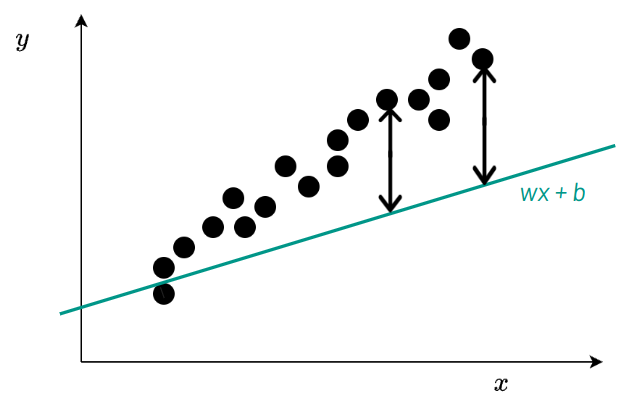
\includegraphics[height=4cm]{figues/modele_lineaire_loss.png}
          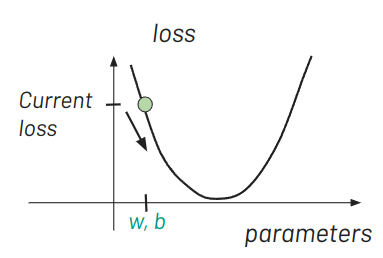
\includegraphics[height=4cm]{figues/loss.png}
          \end{center}
          \caption{Modèle linéaire et modélisation de la \emph{loss}.}
          \label{fig:loss} \end{figure}

L'actualisation des poids passe par la modélisation de la perte en
fonction des paramètres (Fig. \ref{fig:loss2}).

          \begin{figure}[H]
          \begin{center}
          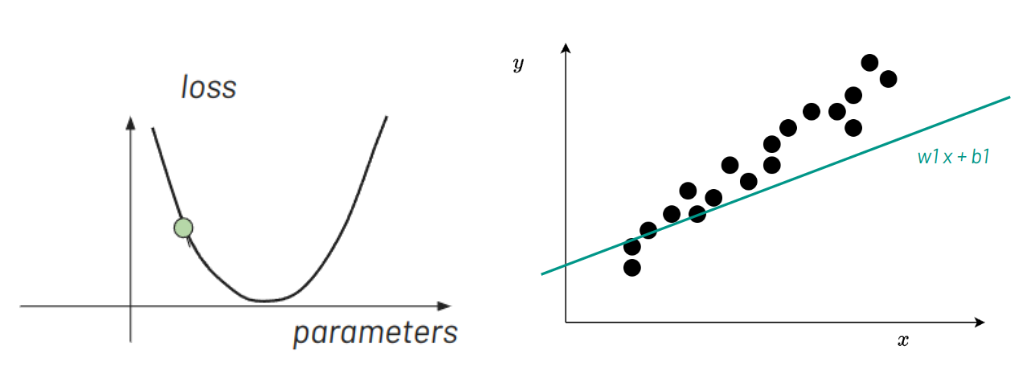
\includegraphics[height=4cm]{figues/modele_lineaire_2.png}
          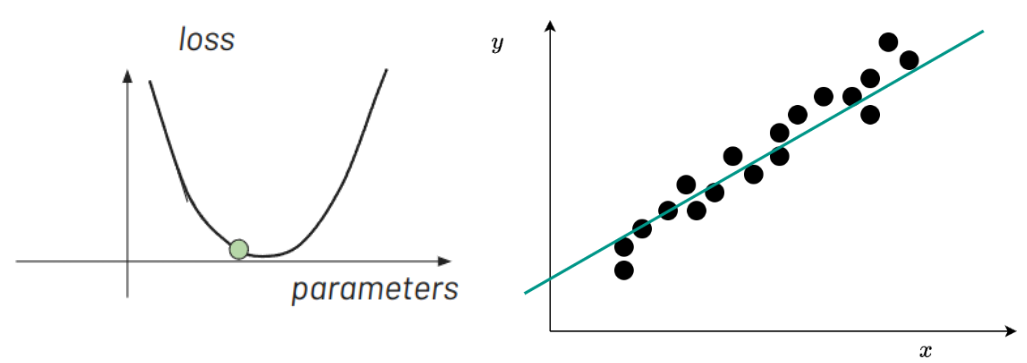
\includegraphics[height=4cm]{figues/modele_lineaire_3.png}
          \end{center}
          \caption{Réduction de la \emph{loss} et ajustement des poids en fonction.}
          \label{fig:loss2} \end{figure}

L'application de cette nouvelle représentation permet de moduler les
paramètres de manière à minimiser la fonction de perte. Le modèle, ainsi
ajusté, génère des prédictions naturellement plus proches des données
d'entraînement. En répétant ce processus de manière itérative, et en
actualisant les paramètres à chaque itération pour réduire la fonction
de perte, on obtient un ensemble de paramètres optimisés qui minimise
efficacement la fonction de perte sur les données d'entraînement. On dit
de ce modèle qu'il est \emph{appris}, et il peut être évalué sur de
nouvelles données (des datapoints inconnus constituant les données de
test).

Ce processus peut être généralisé à un modèle intégrant plusieurs
variables d'entrée~: un modèle linéaire multidimensionnel. En effet, il
serait simpliste de supposer que le prix d'une maison dépend uniquement
de sa superficie. De nombreux facteurs influencent le prix, tels que
l'année de construction et la localisation. Cependant, chaque paramètre
n'exerce pas une influence équivalente sur les prédictions de sortie. Le
modèle doit ainsi considérer la somme pondérée des \emph{n} variables
d'entrée, l'apprentissage consistant à apprendre ces poids, grâce au même processus itératif.

\emph{De l'apprentissage à l'apprentissage profond}

Jusqu'à présent, nous avons abordé des structures mathématiques simples,
représentées par des équations linéaires, qui permettent de modéliser
des relations basiques entre les entrées et la sortie. Pour ces
exemples, il n'est pas nécessaire d'utiliser des architectures
neuronales complexes avec des connexions explicites~: de tels réseaux
(appelée \emph{Multiple Layer Perceptron} ou Perceptron multi-couche) se
composent d'une multiplication et d'association entres ces modèles
linéaires organisés en couches. L'insertion de couches intermédiaires ou
couches cachées (en anglais, hidden layers) entre l'entrée et la sortie
de cette architecture complexe permet de construire des modèles de plus
en plus sophistiqués.

Chaque neurone calcule une somme pondérée des entrées reçues, à laquelle
il applique une fonction d'activation non linéaire, telle que la
fonction sigmoïde, la tangente hyperbolique ou la fonction logistique.
Cette fonction d'activation, appelée activation function, est conçue
pour introduire de la non-linéarité dans le modèle~: elle s'active pour
des sommes pondérées élevées et modère ou annule les activations pour
des sommes plus faibles. Ainsi, est créé un modèle paramétrique
hautement non-linéaire qui permet de capturer des relations complexes et
d'augmenter la capacité du modèle à généraliser à des données plus
variées.

Le principe fondamental de l'apprentissage d'un perceptron multicouche,
connu sous le nom de rétropropagation ou \emph{backpropagation},
correspond au phénomène d'actualisation des poids. Initialement, tous
les poids sont assignés de manière aléatoire. Pour chaque input dans le
jeu de données d'entraînement, le réseau de neurones artificiel est
activé et une sortie est observée. Cette sortie (dite \emph{prédite})
est comparée à la sortie attendue, telle qu'annotée dans les données
d'entraînement. S'il y a erreur, celle-ci est ``propagée'' à la couche
précédente, et les poids sont ajustés en fonction. Le processus se
répète jusqu'à ce que le taux d'erreur en sortie passe sous un
\emph{threshold} prédéterminé.

\emph{L'entraînement}

Il faut distinguer l'algorithme d'apprentissage du modèle appris~: le
premier utilise les données pour produire le second, qui peut ensuite
être appliqué comme un programme classique. Un algorithme
d'apprentissage permet donc de modéliser un phénomène à partir
d'exemples. Un modèle est un objet qui existe à un instant \emph{t}, il
est le résultat de l'entraînement d'un réseau de neurones et ne sera
plus le même après ré-entraînement.

Le terme \emph{entraînement} fait référence à un processus itératif
composé de plusieurs passages à travers le jeu de données, appelés
époques (ou \emph{epochs} en anglais). Au cours de chaque époque, les
poids du modèle sont ajustés en fonction des erreurs observées. Le
modèle module ainsi automatiquement ses poids au fil des itérations. La
conclusion de l'entraînement est atteinte lorsque le modèle atteint un
niveau de performance jugé satisfaisant.

Un modèle est dit ``capable de généraliser'' s'il est capable de
modéliser et capturer des relations complexes entre les données d'entrée
et les données de sortie.

\begin{kwote}                     
``On appelle \emph{généralisation} la capacité d'un modèle à faire des
prédictions correctes sur de nouvelles données, qui n'ont pas été
utilisées pour le construire''.\footcite[p.27]{azencott_introduction_2022}
                 \end{kwote}     

Si le réseau de neurones ``profond'' est un modèle paramétrique dont les
paramètres sont les poids de connection, ce modèle a donc d'autant plus
de poids de connexion (de paramètres) qu'il a de couches intermédiaires
et de neurones dans les couches. Pour éviter qu'ils ne ``colle'' trop
aux données (et soit donc incapable de généraliser\footnote{le phénomène
  d'\emph{overfitting} sera évoqué dans le \hyperlink{fine-tuner-le-modele}{chapitre 5}}),
l'apprentissage de ``bons'' modèles requiert souvent des quantités
massives de data.

Après la phase initiale d'entraînement, il est possible de procéder à un
ré-entraînement ou \emph{fine-tuning}. Cette étape permet de rendre le
modèle plus adapté à des données spécifiques, mais elle n'améliore pas
nécessairement ses performances globales sur la tâche initiale. En
d'autres termes, le ré-entraînement ou l'ajustement fin augmente la
spécialisation du modèle pour des ensembles de données particuliers, ce
qui peut influencer la capacité du modèle à généraliser à de nouveaux
contextes.

Pour conclure, un modèle est avant tout une collection de poids qui
s'adaptent grâce à un algorithme d'apprentissage pour réduire la \textit{loss}.
La phase d'entraînement consiste à tester des paramètres et des liens,
et à affecter une pondération à ces liens. Toutes les pondérations,
pour chaque couche, pour chaque neurone, constitue le modèle. Plus le
phénomène à analyser est complexe plus le modèle est lourd (plus il a de
poids).